\section{Collision Avoidance} \label{sec:collision_avoidance}

\subsection{Disturbance Repulsion}
A crucial property of the passive obstacle-aware controller is its ability to ensure collision avoidance. For this, we analyze the ability and limitations of the proposed controller to absorb disturbances.
Let us assume a disturbance impact at time $t=0$, which results in the robot having a velocity of $\vecs{\dot \xi} = \vect f(\vecs \xi) + \vect v^I$, which is pointing towards the obstacle (see Fig.~\ref{fig:disturbance_with_parallel_velocity}). 
Note that, the Coriolis effect is neglected due to the small motion of the agent.

\begin{lemma}
	A dynamical system evolves with the rigid body dynamics given in \eqref{eq:robot_dynamics} controlled by \eqref{eq:control_command}, with damping matrix $\matd{D}$ from \eqref{eq:damping_summation}, and a negligible Coriolis effect.
    A point-like agent  close to the surface, i.e., $\Gamma( \{ \vecs\xi \}_0) \approx 1$ is guided by a velocity field $\vect f(\vecs \xi)$ parallel to the surface starting at position $\vect p = \{{\vecs \xi}\}_0$ and with velocity $\vect v^0= \vect f(\{{\vecs \xi}\}_0)$.
    A large disturbance towards the obstacle results in a velocity of $\{\dot{\vecs \xi}\}_0 = \vect v^I +  \vect v^0$ after the impact, with $\| \vect v^I \| \gg \| \vect v^0 \|$.
	A motion starting in free space remains collision-free for all times, i.e., $\Gamma( \{\vecs \xi_t\}) \geq 1$ with $t \geq 0$ if the impact velocity is limited as follows $\| \vect v^I\| < s^{\mathrm{o}} \| \vecs \xi - \vecs \xi^b \| / m^{\mathrm{min}}$, with respect to the closes surface point $\vecs \xi^b \in \mathbb{R}^N$ and smallest eigenvalue of the mass matrix $m \in \mathbb{R}_{>0}$.
\end{lemma}


\begin{figure}[htb]
\centering
 % \begin{subfigure}{0.99\columnwidth}
  \centerline{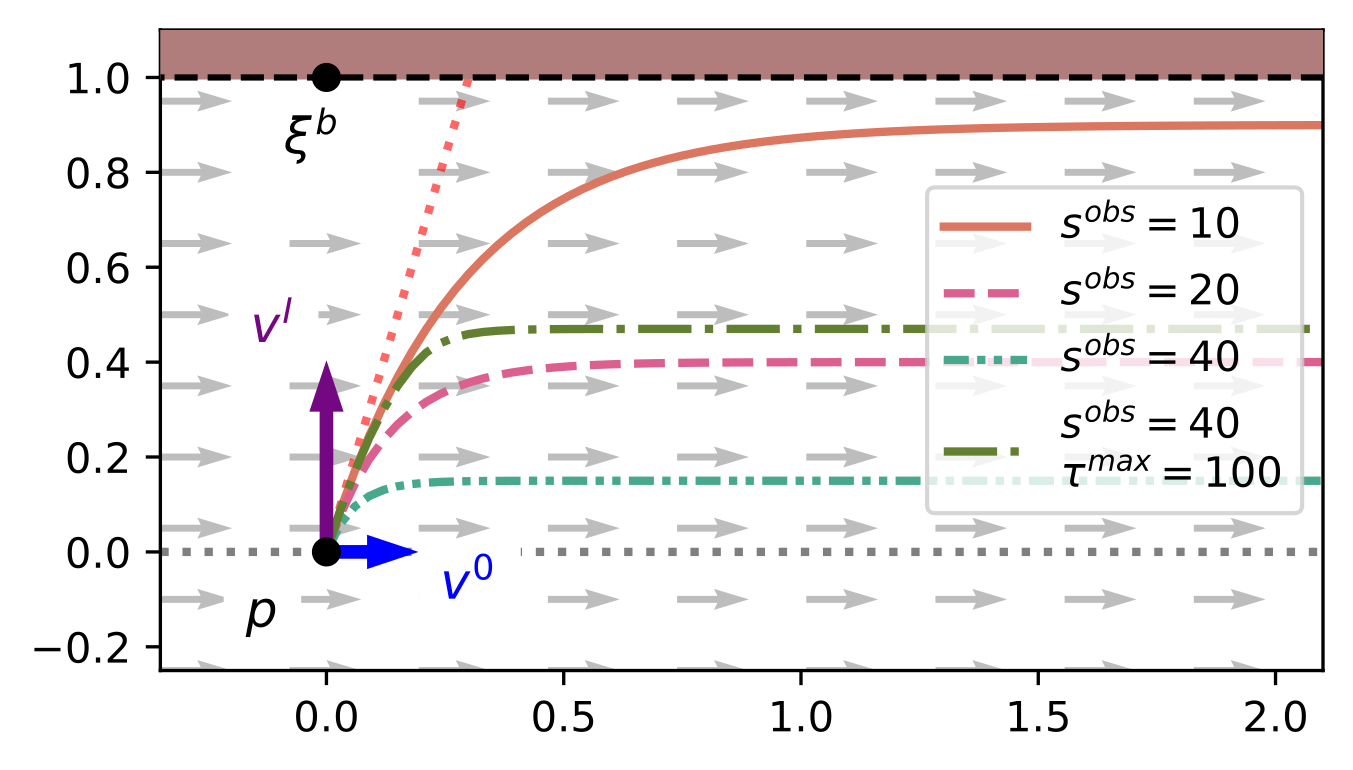
\includegraphics[width=0.99\columnwidth]{figures/parallel_avoidance_obstacle}}
  \caption{Disturbance rejection in the presence of a constant velocity field (blue), and different damping values $s^{\mathrm{o}}$ and optionally a maximum repulsion force $\vecs \tau^{\mathrm{max}}$ for the green trajectory.}
  \label{fig:disturbance_with_parallel_velocity}
% \end{subfigure}
\end{figure}
    
\begin{proof}
Since we assume a point-like agent, the mass matrix $\matd{M}(\vecs \xi)$ is constant. The damping matrix in proximity of a single obstacle is approximated as:
\begin{equation}
\Gamma(\vecs \xi) \approx 1
\; \underset{\eqref{eq:averaged_normal}, \, \eqref{eq:weight_function} } {\Rightarrow} \;
\begin{array}{l}
% \lim_{\Gamma(\vecs \xi) \rightarrow 1} \| \vect n(\vecs \xi) \| = 1, \\
% \lim_{\Gamma(\vecs \xi) \rightarrow 1}\; w(\vecs \xi) = 1
\| \vect n(\vecs \xi) \| = 1 \\
w(\vecs \xi) = 1
\end{array}
% \quad 
\underset{\eqref{eq:damping_summation}} {\Rightarrow} \quad
\matd D(\vecs \xi) = \matd{D}^o(\vecs \xi)
\end{equation}

Using the controller design from \eqref{eq:control_command} the velocity can be computed as:
\begin{equation}
\begin{split}
    \vecs{\dot \xi} & = \int \vecs{\ddot \xi} \, dt 
    = \int \matd{M}^{-1} \matd{D}  \left( \vecs{\dot \xi} - \vecs f(\vecs \xi) \right) \, dt \\
    % & \approx \int \matd{M}^{-1} \matd{D} \vect f(\vecs \xi) \, dt
\end{split}
\label{eq:velocity_evolution}
\end{equation}

Due to the large disturbance towards the obstacle relative to the tangent velocity, i.e., $\| \vect v^I \| \gg \| \vect v^0 \|$, as well as the proximity to the obstacle from $\Gamma(\vecs \xi) \approx 1$, the agent is only able to move little before having to reject the disturbance. 
As a result, we can assume that the changes of the velocity field and the obstacle curvature are negligible, and hence we have $\vect f(\vecs \xi) = \text{const.}$ and $\vect n(\vecs \xi) = \text{const.}$
Hence, using \eqref{eq:obstacle_damping_values} results in a constant damping matrix with damping values:
\begin{equation}
    \matd{S}^o_1 = s^o
    \; , \quad
    \matd{S}^o_2 = s^f
    \; , \quad
    \matd{S}^o_d = s^c \;\;\; d = 3 .. N
\end{equation}
Additionally, the first decomposition vector $\vect q_1^o(\vecs \xi)$ points along the normal $\vect n(\vecs \xi)$, and the second $\vect q_2^o(\vecs \xi)$ along the desired dynamics $\vect f(\vecs \xi)$.

This allows for the analysis of the velocity from \eqref{eq:velocity_evolution} along decomposition direction $q_d^o$. In the tangent plane, the impact did not change the velocity, and hence:
\begin{equation}
\begin{split}
    \dot{\vecs \xi}_d & = \int \matd{M}^{-1} \matd{D}  \left( \vecs f_d(\vecs \xi) - \vecs f_d(\vecs \xi) \right) \, dt  =  \vect v^0_d
    %\qquad \text{with} \quad
\end{split}
\end{equation}
with $d = 2 .. N$.

Conversely, in the direction of the obstacle we have:
\begin{equation}
    \vecs{\dot \xi}_1 = \int \frac{s^{\mathrm{o}}}{m} \vecs{ \dot \xi}_1 \, dt = \frac{s^{\mathrm{o}}}{m} \left(\vecs{\xi}_1 - \vect p_1 \right)  + \vecs v^I_1 \label{eq:velocity_with_control}
\end{equation}
% where $m = \min \Bigl(\text{eig} \bigl(\mathcal{M} \bigr) \Bigr)$ is the smallest eigenvalue of the mass matrix. Note, that any velocity which does not point towards the surface, will not get as close to the obstacle.

This can be used to compute the distance at which the velocity reaches zero:
\begin{equation}
    \| \vecs{\dot \xi} _1 \| = 0
    \quad \Rightarrow \quad
    \| \vecs{\xi}_1 -  \vect p_1 \| = \| \vecs v^I_1 \| {m} / {s^{\mathrm{o}}} 
\end{equation}
Hence, as long as the disturbance is limited by
\begin{equation}
    \| \vect v^I \| < s^{\mathrm{o}} \| \vecs \xi - \vecs \xi^b \| / m
\end{equation}
it will stop at the closest surface point $\vecs \xi^b \in \mathbb{R}^N$. And hence remain collision-free.
\end{proof}

Note that the analysis is done for proximity regions of the obstacle. In any case, the robot enters this proximity region before a collision can occur. Hence, the proposed analysis holds as a general collision avoidance insurance.

So far the disturbance has been in the form of a velocity, yet a system is disturbed by force. The corresponding disturbance velocity is obtained by integrating the force over time (considering the mass matrix).

Furthermore, while here we specifically disturbances only in the direction of the obstacle, any disturbance can be divided into a part towards the obstacle, and a part parallel. Where a disturbance parallel to the obstacle does not pose any danger for collision.
However, the porpoised method does not give any guarantee against drifting into the obstacle, as is discussed during the experiments in the Section~\ref{sec:position_noise}, yet the increased damping towards the obstacle does significantly reduce it. 

% The prove used assumption a constant velocity field and negligible curvature. In case of large disturbances close to the obstacle, such that $\| \vect v^I \| \gg \| \vect f(\vecs \xi) \|$, such an assumption is reasonable, because the relative motion is small, while rejecting the disturbance.

\subsection{Disturbance Repulsion with Force Limit}
All robotic systems have a maximum force that they  exert based on the motors and their geometry, $\tau_c^{\mathrm{max}} \in \mathbb{R}_{>0}$. Note that such a force might be state-dependent.

A limiting force increases the impact velocity $\vect v^I$ a controller can handle to ensure collision avoidance (Fig.~\ref{fig:disturbance_with_parallel_velocity}). Nevertheless, a maximum control force can be interpreted as an adapting damping parameter, and hence, the passivity from Theorem~\ref{theorem:passivity} still holds.


